\documentclass{article}
\usepackage[utf8]{inputenc}
\usepackage[top=1in, bottom=1in, left=1in, right=1in]{geometry}
% \usepackage{indentfirst}
\usepackage{amsmath}
\usepackage{amssymb}
\usepackage{mathtools}
\usepackage{graphicx}
    \DeclareGraphicsExtensions{.png, .jpeg}
\usepackage{caption}

% custom macros
\newcommand*{\doublebar}[1]{\overline{\overline{#1}}}
\newcommand*{\unknown}[0]{\;?\;}
\DeclareMathOperator*{\argmax}{argmax}

% main document
\title{MATH 786: Cooperative Game Theory \\ HW06}
\author{Terence Henriod}
\date{\today}

\begin{document}

\maketitle

\begin{abstract}
Shapley Value, Multi-linear Extensions, House-swapping Games. 
\end{abstract}


\newpage
\begin{enumerate}
\item Consider the three person TU game below:
$N = \{1, 2, 3\}$, $V(\emptyset) = 0$, $V(\overline{1}) = 3$, $V(\overline{2}) = 2$, $V(\overline{3}) = 0$, $V(\overline{1, 2}) = 4$, $V(\overline{1, 3}) = 6$, $V(\overline{2, 3}) = 8$, $V(N) = 10$

  \begin{enumerate}
  \item Find the multilinear extension of the game. \\

  \textit{Solution}: \\

  $g(x_{1}, x_{2}, x_{3}) =
         3x_{1} + 2x_{2} - 1x_{1}x_{2} + 3x_{1}x_{3} + 6x_{2}x_{3} - 3x_{1}x_{2}x_{3}$ \\

  \hfill\newline
  Recall that the multilinear extension of a game is of the form:
  \[ g(x_{1}, \dots x_{n}) = \sum_{S \in 2^{N}}{[(\prod_{i \in S}{x_{i}})(\prod_{i \not\in S}{(1 - x_{i})})V(S)]} \]

  So for a three player game, we have:
  \begin{align*}
  g(x_{1}, x_{2}, x_{3}) &= (1)                 * ((1 - x_{1})(1 - x_{2})(1 - x_{3})) * (0)  &+ \\
                         &  (x_{1})             * ((1 - x_{2})(1 - x_{3}))            * (3)  &+ \\
                         &  (x_{2})             * ((1 - x_{1})(1 - x_{3}))            * (2)  &+ \\
                         &  (x_{3})             * ((1 - x_{1})(1 - x_{2}))            * (0)  &+ \\
                         &  (x_{1} x_{2})       * ((1 - x_{3}))                       * (4)  &+ \\
                         &  (x_{1} x_{3})       * ((1 - x_{2}))                       * (6)  &+ \\
                         &  (x_{2} x_{3})       * ((1 - x_{1}))                       * (8)  &+ \\
                         &  (x_{1} x_{2} x_{3}) * (1)                                 * (10) &+ \\
                         %
                         & & \\
                         &=  3x_{1} - 3x_{1}x_{2} - 3x_{1}x_{3}       + 3x_{1}x_{2}x_{3}  &+ \\
                         &   2x_{2} - 2x_{1}x_{2} - 2x_{2}x_{3}       + 2x_{1}x_{2}x_{3}  &+ \\
                         &   4x_{1}x_{2}          - 4x_{1}x_{2}x_{3}                      &+ \\
                         &   6x_{1}x_{3}          - 6x_{1}x_{2}x_{3}                      &+ \\
                         &   8x_{2}x_{3}          - 8x_{1}x_{2}x_{3}                      &+ \\
                         &   10x_{1}x_{2}x_{3}                                            &+ \\
                         %
                         & & \\
                         &=  3x_{1} + 2x_{2} - 1x_{1}x_{2} + 3x_{1}x_{3} + 6x_{2}x_{3} - 3x_{1}x_{2}x_{3}  & \\
  \end{align*}

  %
  \item Use the multilinear extension to find the Shapley Value of the game. \\

  \textit{Solution}: \\

  $\varphi = (\frac{6}{2}, \frac{7}{2}, \frac{7}{2})$ \\

  Recall that:
  \[ \varphi_{i} = \int_{0}^{1} \frac{\partial g}{\partial x_{1}} (t, \dots, t) \partial t \]

  For the $\frac{\partial g}{\partial x_{i}}$s we have:
  \begin{align*}
  \frac{\partial g}{\partial x_{1}} &= 3      - x_{2}  + 3x_{3}      - 3x_{2}x_{3}  \\
  \frac{\partial g}{\partial x_{2}} &= 2      - x_{1}  + 6x_{3}      - 3x_{1}x_{3}  \\
  \frac{\partial g}{\partial x_{3}} &= 3x_{1} + 6x_{2} - 3x_{1}x_{2}
  \end{align*}

  Thus:
  \begin{align*}
  \varphi_{1} &= \int_{0}^{1} \frac{\partial g}{\partial x_{1}} (t, t, t) \partial t \\ 
              &= \int_{0}^{1} 3 - x_{2}  + 3x_{3} - 3x_{2}x_{3} \Big|_{t, t, t} \partial t \\ 
              &= \int_{0}^{1} 3 - t  + 3t - 3t^{2} \partial t \\ 
              &= \int_{0}^{1} 3 + 2t - 3t^{2} \partial t \\ 
              &= 3t + t^{2}  - t^{3} \Big|_{0}^{1} \\ 
              &= 3(1) + (1)^{2} - (1)^{3} - 3(0) - (0)^{2} + (0)^{3} \\ 
              &= 3 + 1 - 1 \\ 
              &= 3 = \frac{6}{2}
  \end{align*}
  \begin{align*}
  \varphi_{2} &= \int_{0}^{1} \frac{\partial g}{\partial x_{2}} (t, t, t) \partial t \\ 
              &= \int_{0}^{1} 2 - x_{1}  + 6x_{3} - 3x_{1}x_{3} \Big|_{t, t, t} \partial t \\ 
              &= \int_{0}^{1} 2 - t  + 6t - 3t^{2} \partial t \\ 
              &= \int_{0}^{1} 2 + 5t - 3t^{2} \partial t \\ 
              &= 2t + \frac{5}{2}t^{2}  - t^{3} \Big|_{0}^{1} \\ 
              &= 2(1) + \frac{5}{2}(1)^{2} - (1)^{3} - 2(0) - \frac{5}{2}(0)^{2} + (0)^{3} \\ 
              &= 2 + \frac{5}{2} - 1 \\ 
              &= \frac{7}{2}
  \end{align*}
  \begin{align*}
  \varphi_{3} &= \int_{0}^{1} \frac{\partial g}{\partial x_{3}} (t, t, t) \partial t \\ 
              &= \int_{0}^{1} 3x_{1}  + 6x_{2} - 3x_{1}x_{2} \Big|_{t, t, t} \partial t \\ 
              &= \int_{0}^{1} 3t  + 6t - 3t^{2} \partial t \\ 
              &= \int_{0}^{1} 9t - 3t^{2} \partial t \\ 
              &= \frac{9}{2}t^{2}  - t^{3} \Big|_{0}^{1} \\ 
              &= \frac{9}{2}(1)^{2} - (1)^{3} - \frac{9}{2}(0)^{2} + (0)^{3} \\ 
              &= \frac{9}{2} - 1 \\ 
              &= \frac{7}{2}
  \end{align*}

  Note, that on the previous homework we found the same Shapley Value ($\varphi = (\frac{6}{2}, \frac{7}{2}, \frac{7}{2})$) for the same game using the combinatoric method. \\
  %
  \end{enumerate}

%
\item Consider the eight person houseswapping game (with strict preferences):
\begin{align*}
1: 2,3,4,5,6,7,8,1 \\
2: 3,5,6,7,1,8,4,2 \\
3: 6,1,2,8,5,3,4,7 \\
4: 4,3,5,6,1,7,8,2 \\
5: 3,2,1,4,7,8,6,5 \\
6: 4,1,3,5,6,7,8,2 \\
7: 2,3,5,7,4,6,8,1 \\
8: 1,6,2,3,5,4,7,8 \\
\end{align*}

  \begin{enumerate}
  \item Find the unique strict core permutation of this game. \\

  \textit{Solution}: \\
  
  $\Pi^{*} = \{ 1 \rightarrow 2,\; 2 \rightarrow 3,\; 3 \rightarrow 6,\; 4 \rightarrow 4,\; 5 \rightarrow 7,\; 6 \rightarrow 1,\; 7 \rightarrow 5,\; 8 \rightarrow 8 \}$ \\

  The Top Trade Cycle (TTC) Algorithm gives the a permutation in the strict core of a house-swapping game, so using that should be sufficient: \\

  \begin{tabular}{| c | c | c | c | c |}
  \hline
  $i$ & $N - P$ & Graph & TCCs & $P$ \\
  \hline\hline
  1   & $1, 2, 3, 4, 5, 6, 7, 8$ & 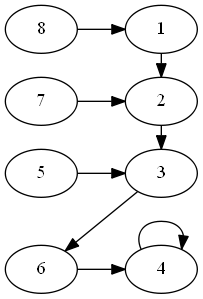
\includegraphics[scale=0.3]{step-1}
            & $4 \rightarrow 4$ & $4$ \\
  \hline
  2   & $1, 2, 3, 5, 6, 7, 8$ & 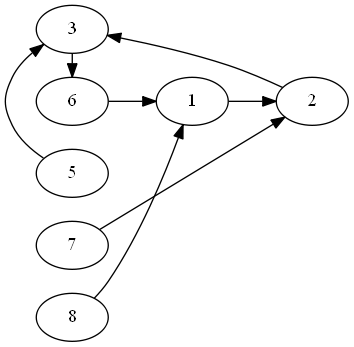
\includegraphics[scale=0.3]{step-2}
            & $1 \rightarrow 2 \rightarrow 3 \rightarrow 6 \rightarrow 1$ & $1, 2, 3, 4, 6$ \\
  \hline
  3   & $5, 7, 8$ & 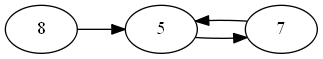
\includegraphics[scale=0.3]{step-3}
            & $5 \rightarrow 7 \rightarrow 5$ & $1, 2, 3, 4, 5, 6, 7$ \\
  \hline
  4   & $8$ & 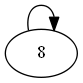
\includegraphics[scale=0.3]{step-4}
            & $8 \rightarrow 8$ & $1, 2, 3, 4, 5, 6, 7, 8$ \\
  \hline
  \end{tabular} \\

  %
  \item Find a core permutation which is not in the strict core. \\

  \textit{Solution}: \\
  
  $\Pi^{*} = \{ 1 \rightarrow 2,\; 2 \rightarrow 3,\; 3 \rightarrow 6,\; 4 \rightarrow 4,\; 5 \rightarrow 8,\; 6 \rightarrow 1,\; 7 \rightarrow 5,\; 8 \rightarrow 7 \}$ \\
  
  In order for a permutation $\hat{\Pi}$ to be in the core, the permutation must satisfy
  \[ \nexists \; \Pi,\, S \quad s.t. \quad \begin{cases} \Pi(S) = S \\
                             \Pi(i) \succ^{i} \hat{\Pi}(i) \quad \forall i \in S
     \end{cases} \]
  For the permutation to be in the strict core, the requirement is added that no coalition can ``weakly block" the grand coalition, meaning that a coalition cannnot exist where all of the players are no worse off than in the grand coalition, but at least one player is strictly better off. So we need to find a weakly blocking coalition for our non-strict core permutation in addition to finding a permutation meeting the above conditions. \\

  We can alter the strict core solution to achieve a permutation that contains a weakly blocking coalition but is still in the core, but not in the strict core. \\

  When we consider players $1, 2, 3, 4$, these will not be in the weakly blocking coalition because they got their first choice, and being in a weakly blocking coalition would mean that they would either need to have this allocation improved upon, or their house would have to improve on the original owner of their first choice house. This is not possible for any of these players as their houses go to players who also get their first choice of house. This, of course, requires to look to $6$, whose house is $3$'s first choice, but $6$ gets their best possible choice after $4$ gets their house, so $6$ is in a very similar situation as $1, 2, 3, 4$ - none of these players can give their house to another player to improve their situation without taking a worse house. \\

   An educated guess (by examining all permutations of the remaining players: $5, 7, 8$) says that we can trade the houses that $5$ and $8$ get in the strict core permutation, giving $\Pi^{*} = \{ 1 \rightarrow 2,\; 2 \rightarrow 3,\; 3 \rightarrow 6,\; 4 \rightarrow 4,\; 5 \rightarrow 8,\; 6 \rightarrow 1,\; 7 \rightarrow 5,\; 8 \rightarrow 7 \}$. This permutation leaves $5$ worse off, but $8$ better off; individual rationality is maintained and no permutation of any coalition fares strictly better than in this permutation. \\

  Now consider the coalition $\overline{5, 7}$. As a coalition, these players could use the allocation $5 \rightarrow 7 \rightarrow 5$, which leaves $5$ with a more preferable house, but $7$ remains the same. $\overline{5, 7}$ is our weakly blocking coalition. \\

  The permutation is in the core, but can be weakly blocked, so it is a permutation satisfying the requirements. \\
  %
  \end{enumerate}

%
\item Find an $n$-player houseswapping game in which, when the TTC algorithm is run:

  \begin{enumerate}
  \item the algorithm runs for ONE iteration, but one obtains $n$ distinct TTCs. \\

  \textit{Solution}: \\

  The game has $N = \{1, \dots, n\}$ and $\succ$ is defined such that each player most prefers their own house (the remaining preferences can be any allowable possibility without any difference to the outcome of the algorithm. \\

  This game will produce $n$ distinct TTCs in one iteration because in the first iteration, the graph will consist of every vertex having a self arc and nothing more. \\

  %
  \item The algorithm runs for $n$ iterations, and one obtains $n$ distinct TTCs. \\

  \textit{Solution}: \\

  The game has $N = \{1, \dots, n\}$ and $\succ$ is defined such that each player's $i^{th}$ preference is house $i$. \\

  In each iteration, only one cycle will be formed: the cycle of a player $i$'s self-arc, thus only one player will be eliminated for consideration and one cycle detected with each iteration. (Note: technically, player $m$'s $(m + 1)^{th}$ preferences and beyond may be arbitrary as long as they are legal since the player is removed from further consideration after iteration $m$) \\

  %
  \end{enumerate}

%
\item Suppose we consider houseswapping games WITH INDIFFERENCES ALLOWED, i.e., traders are allowed to be indifferent between houses. Consider the following two examples:

A)
\begin{align*}
T_{1} = 2 \sim 3 \succ 1 \\
T_{2} = 1 \sim 3 \succ 2 \\
T_{3} = 1 \sim 2 \succ 3
\end{align*}

B)
\begin{align*}
T_{1} = 2 \succ 3 \succ 1 \\
T_{2} = 1 \sim  3 \succ 2 \\
T_{3} = 1 \succ 2 \succ 3
\end{align*}

  \begin{enumerate}
  \item Find the set of strict core permutations in both examples. Is it true, in the houseswapping game with indifferences allowed that the strict core still always consists of a single permutation? \\

  \textit{Solution}: \\

  For A) the strict core is the set of the permutations
  \[ \{\Pi^{*}: \Pi^{*} = \{1 \rightarrow 2,\, 2 \rightarrow 3,\, 3 \rightarrow 1\} \text{ or }
                \{1 \rightarrow 3,\, 2 \rightarrow 1,\, 3 \rightarrow 2\} \} \]
  For B) the strict core is empty. \\
  The strict core will not always consist of a single permutation when indifferences are allowed. \\

  We can apply the TTC algorithm, and in the case of an indifference put multiple arcs in the graph for a player's preferences (since an indifference between two choices could be interpreted as having multiple first choices). \\

  For A) we have: \\
  \begin{tabular}{| c | c | c | c | c |}
  \hline
  $i$ & $N - P$ & Graph & TCCs & $P$ \\
  \hline\hline
  1   & $1, 2, 3$ & 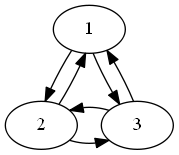
\includegraphics[scale=0.4]{HW06-4-A-1}
            & $1 \rightarrow 2 \rightarrow 3 \rightarrow 1$ or $1 \rightarrow 3 \rightarrow 2 \rightarrow 1$ & $1, 2, 3$ \\
  \hline
  \end{tabular} \\

  There are two largest possible cycles (both are a complete tour of the graph), so there are two permutations that give all players a house that would be their ``first choice". \\

  For B) we have: \\
  \begin{tabular}{| c | c | c | c | c |}
  \hline
  $i$ & $N - P$ & Graph & TCCs & $P$ \\
  \hline\hline
  1   & $1, 2, 3$ & 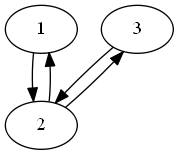
\includegraphics[scale=0.4]{HW06-4-B-1}
            & $1 \rightarrow 2 \rightarrow 1$ or $2 \rightarrow 3 \rightarrow 2$ & $1, 2$ or $2, 3$ \\
  \hline
  2   & $1$ or $3$ & 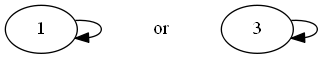
\includegraphics[scale=0.4]{HW06-4-B-2}
            & $3 \rightarrow 3$ or $1 \rightarrow 1$ & $1, 2, 3$ \\
  \hline
  \end{tabular} \\

  however, note that in B), the resulting permutations cannot be strict since they can be weakly blocked, $\Pi^{*} = \{1 \rightarrow 2,\, 2 \rightarrow 1,\, 3 \rightarrow 3\}$ is weakly blocked by the coalition $\overline{2, 3}$ because $3$ could have their first choice while $2$ will still get a first choice, and $\Pi^{*} = \{1 \rightarrow 1,\, 2 \rightarrow 3,\, 3 \rightarrow 2\}$ is weakly blocked by $\overline{1, 2}$ by similar logic. \\

  %
  \item Suppose we run the TTC algorithm on example B), breaking ``ties" arbitrarily. What property does the output have? \\

  \textit{Solution}: \\

  The output of the TTC algorithm with B) as input has the property that the output permutation is in the non-strict core. Neither of the permutations are in the strict core because either permutation can be weakly blocked. $\Pi^{*} = \{1 \rightarrow 2,\, 2 \rightarrow 1,\, 3 \rightarrow 3\}$ is weakly blocked by the coalition $\overline{2, 3}$ because $3$'s situation improves while $2$'s will stay the same, and $\Pi^{*} = \{1 \rightarrow 1,\, 2 \rightarrow 3,\, 3 \rightarrow 2\}$ is weakly blocked by $\overline{1, 2}$ by similar logic. \\

  We could also say that no matter which way the ``tie" is broken, the output still contains the same number of TTCs, the same numbers of players get their $n^{th}$ choices, and so forth. \\
  %
  \end{enumerate}
%
\end{enumerate}
%
\end{document}
